\section{An�lisis}\label{sec:discusion}

\subsection{}\label{subsec:analisis-1}

Las figuras~\ref{fig:d1},~\ref{fig:d2},~\ref{fig:d3},~\ref{fig:d4} y~\ref{fig:d5} representan las rectas $\tan{\alpha}$ frente a la intensidad $I$
para las distintas distancias $d$\footnote{En las figuras se emplea la notaci�n anglosajona, donde se utiliza el punto como separador de decimales.
}.

\FloatBarrier

\begin{figure}[h!]
    \begin{center}
        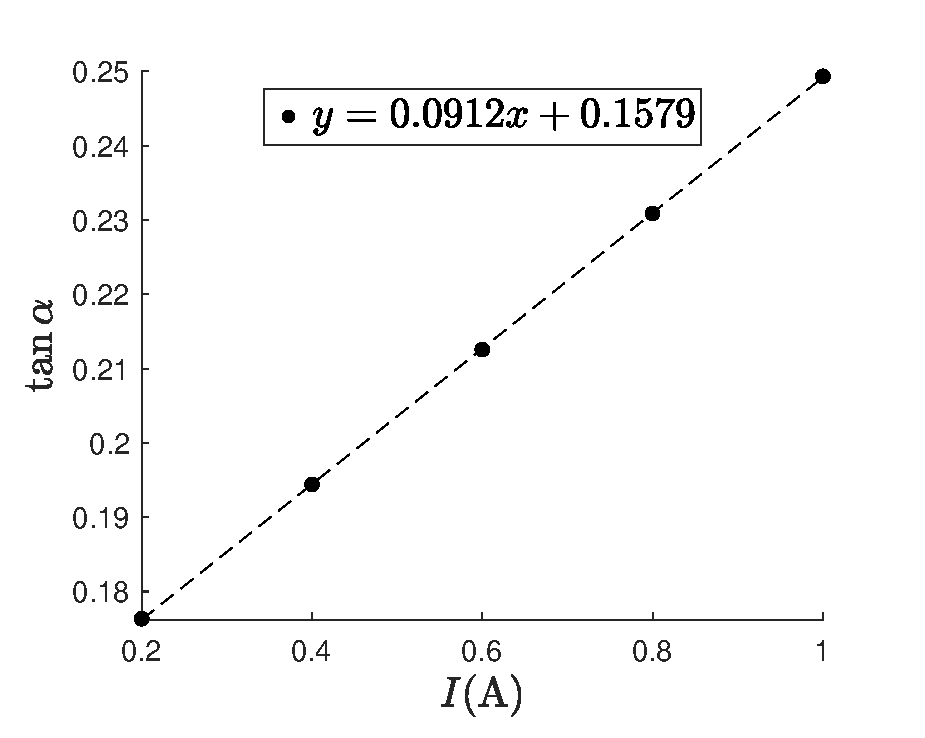
\includegraphics[width=0.8\columnwidth]{files/images/d1}
    \end{center}
    \caption{$\tan{\alpha}$ frente a $I$ para $d = 5\,$cm.}
    \label{fig:d1}
\end{figure}

\FloatBarrier

\begin{figure}[h!]
    \begin{center}
        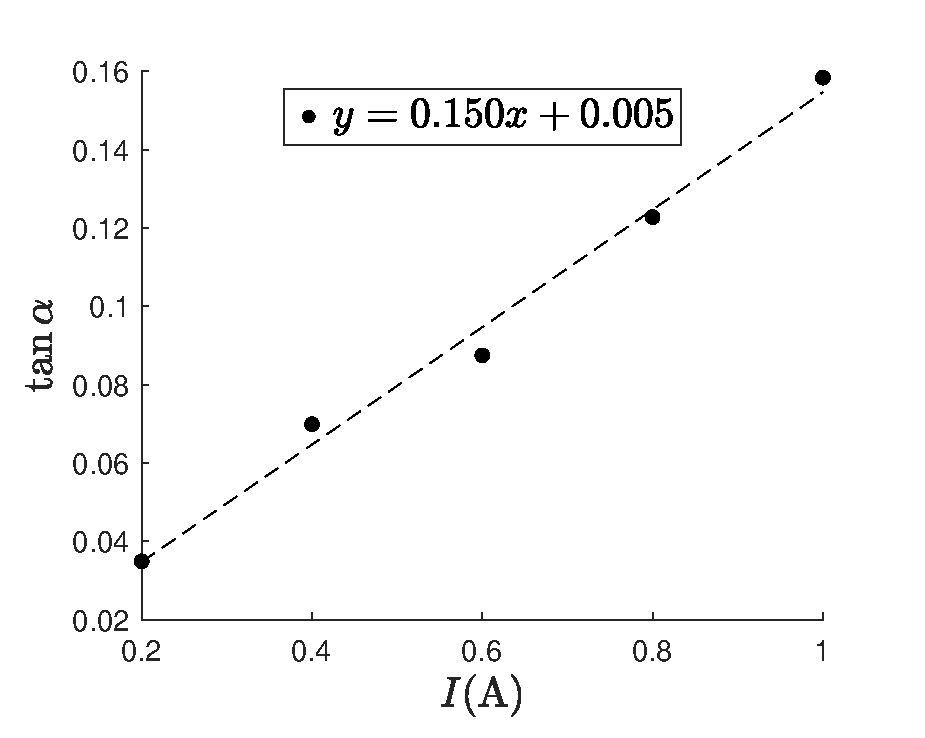
\includegraphics[width=0.8\columnwidth]{files/images/d2}
    \end{center}
    \caption{$\tan{\alpha}$ frente a $I$ para $d = 10\,$cm.}
    \label{fig:d2}
\end{figure}

\begin{figure}[h!]
    \begin{center}
        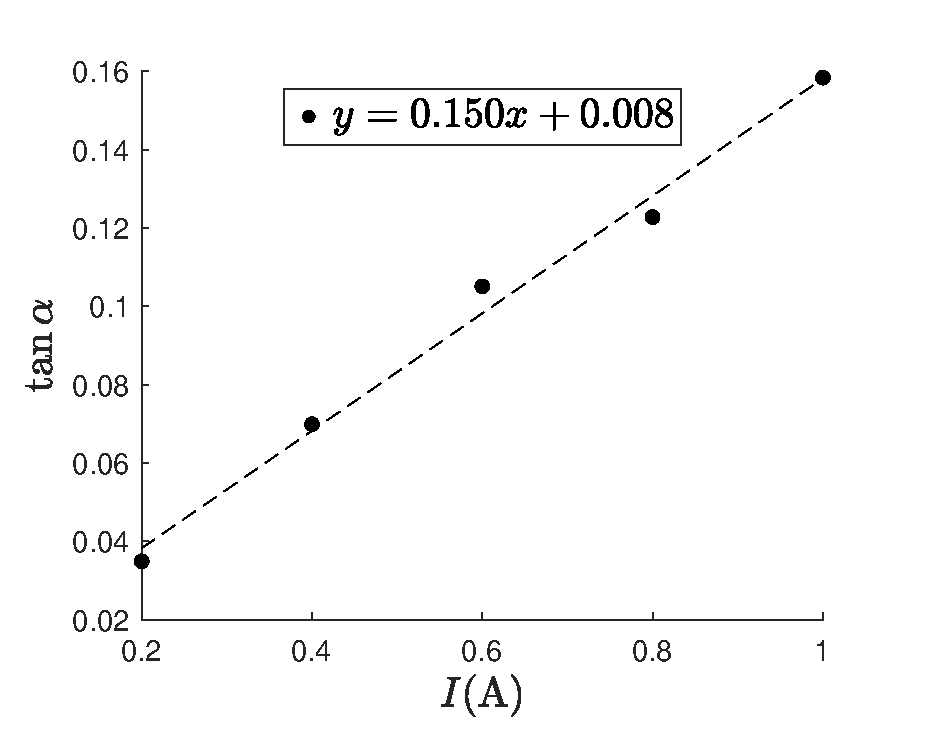
\includegraphics[width=0.8\columnwidth]{files/images/d3}
    \end{center}
    \caption{$\tan{\alpha}$ frente a $I$ para $d = 15\,$cm.}
    \label{fig:d3}
\end{figure}

\FloatBarrier

\begin{figure}[h!]
    \begin{center}
        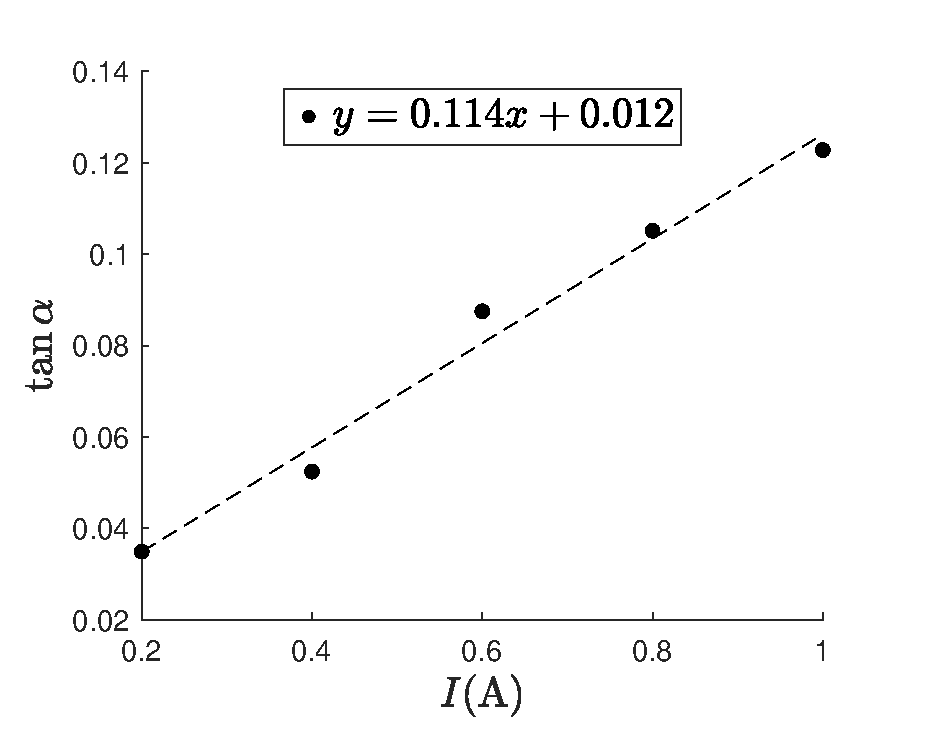
\includegraphics[width=0.8\columnwidth]{files/images/d4}
    \end{center}
    \caption{$\tan{\alpha}$ frente a $I$ para $d = 20\,$cm.}
    \label{fig:d4}
\end{figure}

\begin{figure}[h!]
    \begin{center}
        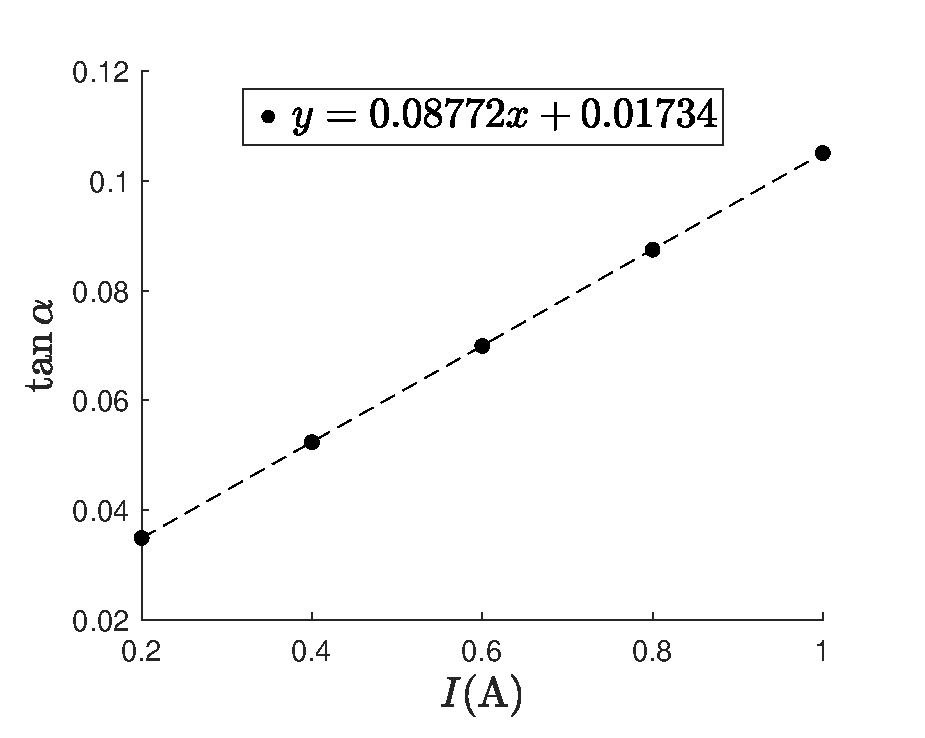
\includegraphics[width=0.8\columnwidth]{files/images/d5}
    \end{center}
    \caption{$\tan{\alpha}$ frente a $I$ para $d = 25\,$cm.}
    \label{fig:d5}
\end{figure}


Seg�n la ecuaci�n~\ref{eq:tangente}, la pendiente de las rectas es:
\begin{equation}
    \label{eq:a}
    a = \frac{\mu_0}{2\pi d H}
\end{equation}

Se puede calcular el valor de la componente horizontal del campo magn�tico terrestre despejando $H$ en la ecuaci�n anterior.

Los valores se recogen en la tabla~\ref{tab:a}.

\begin{table}[h!]
    \center
    \caption{Componente horizontal del campo magn�tico terrestre $H$ calculada para diferentes distancias $d$.}
    \label{tab:a}
    \begin{centering}
        \begin{tabular}{|P{30px}|P{82px}|P{50px}|}
            \hline
            $d\,$(cm) & $a$       & $H\,$(\mu T)                         \\
            \hline
            \csvreader[no head,late after line= \\, /csv/separator=semicolon ]{./files/data/a_H.csv}{}% use head of csv as column names
            {\csvcoli & \csvcolii & \csvcolv}% specify your columns here
            \hline
        \end{tabular}
    \end{centering}
\end{table}

El error en las medidas de $H$ en la tabla~\ref{tab:a} se ha determinado mediante la expresi�n:
\begin{equation*}
    \epsilon_H = \frac{\mu_0}{2 \pi a d} \Bigl( \frac{\epsilon_d }{d} + \frac{\epsilon_a}{a}   \Bigr)
\end{equation*}

\FloatBarrier

\subsection{}\label{subsec:analisis-2}

La tabla~\ref{tab:k} muestra el valor constante $k = a \, d$.

\begin{table}[h!]
    \center
    \caption{Valor constante $a\, d$.}
    \label{tab:k}
    \begin{centering}
        \begin{tabular}{|P{70px}|}
            \hline
            $k = a \, d\,$(m/A)                 \\
            \hline
            \csvreader[no head,late after line= \\, /csv/separator=semicolon ]{./files/data/a_H.csv}{}% use head of csv as column names
            {\csvcolvi}% specify your columns here
            \hline
        \end{tabular}
    \end{centering}
\end{table}

\FloatBarrier

Seg�n la ecuaci�n~\ref{eq:a}, podemos calcular la componente horizontal del campo magn�tico terrestre $H$ a partir de la constante $k$.
El error de $H$ lo proporciona la dispersi�n de los datos de $k$.

El valor de $H$ obtenido por este m�todo es:
\begin{equation*}
    H = (50 \pm 30)\,\mu\text{T}
\end{equation*}

\subsection{}\label{subsec:analisis-3}

Consultando la referencia~\cite{1}, en la localidad de Calatayud, donde se llev� a cabo esta pr�ctica, el valor de la componente horizontal
del campo magn�tico terrestre es:
\begin{equation*}
    H = 25.2\,\mu\text{T}
\end{equation*}
